\documentclass[tikz,border=5pt]{standalone}
\usepackage[utf8]{inputenc}
\usepackage[T1]{fontenc}
\usepackage{lmodern,amsmath,amssymb}
\usepackage[american]{circuitikz}
\usepackage{pgfplots}
\pgfplotsset{compat=1.18}
\usetikzlibrary{circuits.logic.US,positioning,calc,arrows.meta,patterns,shapes.geometric}
\definecolor{Primary}{HTML}{1F77B4}
\begin{document}
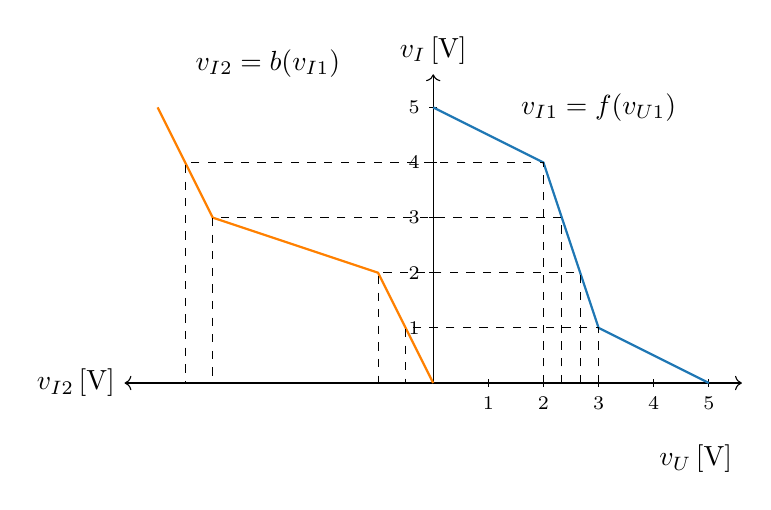
\begin{tikzpicture}[scale=.7]\draw[->] (0,0)--(5.6,0);\node[anchor=north east]at(5.6,-.95){$v_U\,[\mathrm V]$};\draw[->] (0,0)--(0,5.6) node[above]{$v_I\,[\mathrm V]$};\foreach \x in {1,...,5}{\draw (\x,.07)--(\x,-.07) node[below,font=\scriptsize]{\x};\draw (.07,\x)--(-.07,\x) node[left,font=\scriptsize]{\x};}\draw[Primary,thick] (0,5)--(2,4)--(3,1)--(5,0);\draw[->](0,0)--(-5.6,0)node[left]{$v_{I2}\,[\mathrm V]$};\draw[orange,thick](0,0)--(-1,2)--(-4,3)--(-5,5);\foreach\x/\z/\y in{2/4/4.5,2.333333/3/4,2.666667/2/1,3/1/.5}{\draw[dashed](\x,0)--(\x,\z)--(-\y,\z)--(-\y,0);}\node at(3,5){$v_{I1}=f(v_{U1})$};\node at(-3,5.8){$v_{I2}=b(v_{I1})$};\end{tikzpicture}
\end{document}
